\subsection{Resoluci\'on}

En nuestra heurística de búsqueda local decidimos tomar la solución desde la que partimos y mejorarla tomando el primer nodo $nodo1$ y moviéndolo a otro conjunto, verificando aquí si la solución del peso total de todos los conjuntos mejora o empeora (tomándonos la libertad de decir que empeora aun si el peso total es el mismo). Si empeora continuamos de la solución que ya teníamos tomando el próximo nodo, $nodo2$ y repitiendo el mismo proceso de probarlo el los demás conjuntos. En caso de que la solución mejore guardamos el nodo que genera esta mejora y el conjunto al que se debería mover. Una vez que se realizo este proceso en todos los nodos terminaremos teniendo una solución mejor o en el peor caso la misma con la que empezamos.
Si la solución pudo ser mejorada, tomamos esta y se vuelve a ejecutar este procedimiento para esta nueva solución hasta que se llegue a una solución que no puede ser mejorada (mediante esta heurística).
Como se puede notar para cada solución factible definimos el conjunto de soluciones "vecinas" como: aquellas en las que difiere la posición de un solo nodo sobre los k conjuntos, iterando sobre estas hasta hallar la mejora de forma mayoritaria la solución. Esto se repite hasta que se encuentra un valor máximo local (máximo en cuanto a la optimalidad de la solución) que corresponde al mínimo peso obtenido.

Pensamos también plantear la misma solución cambiando la vecindad de soluciones, en esta nueva heurística los vecinos no son las soluciones que difieren en la posición de un nodo, sino que los vecinos los tomamos como aquellos en los que la diferencia se da por el switcheo de dos nodos que pertenecen a distintos conjuntos.
Finalmente descartamos esta segunda heuristica porque presentaba muchos casos desfavorables, por ejemplo la solucion inicial que tiene a todos los nodos en un solo conjunto, como la vecindad esta en intercambiar dos nodos, no podremos sacar ninguno de donde estan. O asi mismo una solucion que presente uno de los k conjuntos vacios. Nunca se podrian agregar nodos a este..

A modo de ejemplo presentamos una demostración gráfica de la heurística.


Partimos de la siguiente solución (1)
\begin{figure}[H]
\begin{center}
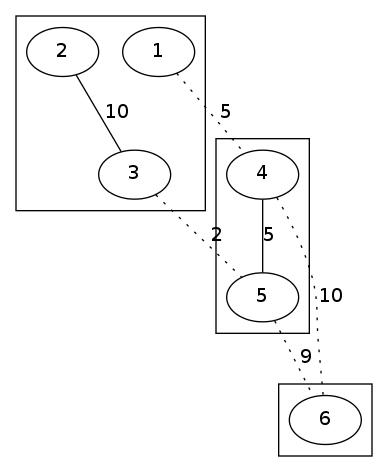
\includegraphics[scale=0.4]{./img/local1.png}
\caption{(1) Solución inicial con k=3}
\end{center}
\end{figure}

A partir de ahora verificara si moviendo un nodo de conjunto puede llegar a una mejor solución, en este momento la suma de los pesos de las aristas intraparticion es igual a 15. Moviendo el nodo $1$ a cualquiera de los otros dos conjuntos no se logra disminuir el peso total, por lo que queda donde esta, ahora el nodo $2$ logra disminuir en 10 moviéndolo a cualquiera de los dos conjuntos restantes, se decide moverlo al segundo. (2)

\begin{figure}[H]
\begin{center}
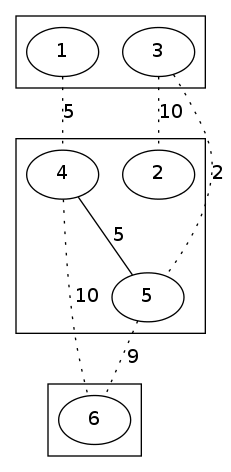
\includegraphics[scale=0.4]{./img/local2.png}
\caption{(2) Solución vecina habiendo movido el nodo $2$}
\end{center}
\end{figure}


Ahora el nodo $3$ aumenta el peso total si se mueve al siguiente conjunto y no aporta nada moverlo al ultimo, por lo que queda en el conjunto en el que está. Lo mismo pasa con el nodo $4$, moviéndolo a uno aumenta el peso y al otro se mantiene. Sigue el nodo $5$ que si se mueve al conjunto donde están los nodos $1$ y $3$ disminuye el peso total a 2, y si se mueve al conjunto restante aumenta el peso en 5, por lo que se ubica en el primer conjunto. Finalmente el nodo $6$ no produce cambios de peso favorables moviéndolo, por lo que la solución a la que llega la heurística es la de la figura (3).

\begin{figure}[H]
\begin{center}
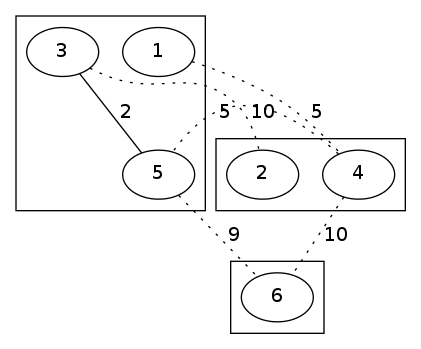
\includegraphics[scale=0.4]{./img/local3.png}
\caption{(3) Solución vecina habiendo movido el nodo $5$ a partir de la solución (2).}
\end{center}
\end{figure}

Habiendo encontrado la solución (3) se llama al recursivamente y se vuelve a realizar el mismo procedimiento. En este caso los nodos $1$, $2$, $3$ y $4$ no mejoran el peso moviéndose de donde están, en cambio el nodo $5$ logra encontrar un peso menor moviéndose al conjunto donde se encuentra el nodo $6$ siendo este cero. Al encontrar una solución óptima ningún movimiento podrá mejorarla, razón por la cual la solución final es la que muestra la imagen (4). 

\begin{figure}[H]
\begin{center}
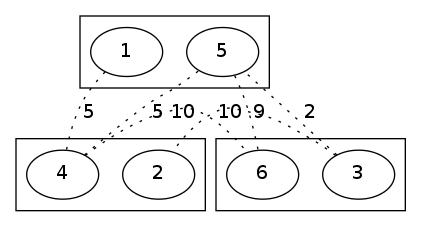
\includegraphics[scale=0.4]{./img/local4.png}
\caption{(4) Solución máxima local.}
\end{center}
\end{figure}

A continuación presentamos un pseudo-gráfico del algoritmo realizado:

\begin{itemize}
\item RESOLVER
	\begin{itemize}
	\item Para cada vértice $v$
		\begin{itemize}
		\item Para cada partición $p$
			\begin{itemize}
			\item Si $v$ esta en la partición $k$, Se calcula cuanto peso 'perdería' restando las aristas intraparticion que inciden en $k$
			\item Sino se calcula cuanto peso 'sumaria' mover $v$ a $p$ guardando el peso, $v$ y $p$ si suma menos peso que con los $v$ y $p$ anteriores (recursión).
			\end{itemize}
		\item Si se llego a una solución mejor, se guarda
		\end{itemize}
	\item Si se encontró alguna solución mejor a la inicial se la toma y se llama recursivamente a RESOLVER con esta.
	\end{itemize}
\end{itemize}


\subsection{Análisis de complejidad}

Para analizar la complejidad del algoritmo de busqueda local vamos a centrarnos en calcular el orden de complejidad temporal de peor caso de una iteracion.
Asi, en cada iteracion de la llamada recursiva de nuestro algoritmo recorremos cada vertice $v$, y por cada vertice, cada particion $p$ asi que hasta aqui tenemos una complejidad en el orden de $O(n.k)$
Dentro de estos dos ciclos se hace lo siguiente.
\begin{itemize}
\item Si $v$ esta en la partición $k$, Se calcula cuanto peso 'perdería' restando las aristas intraparticion que inciden en $k$ (1)
\item Sino se calcula cuanto peso 'sumaria' mover $v$ a $p$ guardando el peso, $v$ y $p$ si suma menos peso que con los $v$ y $p$ anteriores. (2)
\end{itemize}
En el punto (1) en el peor caso, cuando todas las aristas esten en un mismo conjunto, esto tiene un costo igual a $O(m)$. con $m$ cantidad de aristas.  En el punto (2) pasa lo mismo que en el anterior, cuando todas las aristas esten en el mismo conjunto, esto tiene un costo del orden de $O(m)$.
Pero en ambos casos, que son complementarios (sumar o restar las aristas que inciden en $v$ del mismo conjunto) al ejecutarse dentro de la iteracion por cada particion no hace una complejidad de $O(k.m)$ ya que el valor $m$ está amortizado, porque por cada particion no se realizaran $m$ calculos, sino que en el peor caso (porque no todas las aritas incidentes en $v$ son necesariamente intraparticion) se analizarán las $m$ aristas una vez recorridos los $k$ conjuntos, por lo que finalmente esto tiene una complejidad de $O(k+m)$, y en total cada recursion del algoritmo tiene una complejidad en el orden de $O(n.(k+m))$.




\begin{itemize}
\item
\end{itemize}